\chapter{Appendix}\label{chapter:Appendix}

\section{Additional Details to LRP Rules and CRP Implementation}
\label{appendix:lrprules}
In our experiments we follow the recommendations for the application of LRP and CRP as put forward by \cite{Bach2015, Kohlbrenner2020, Montavon2019, Samek2021}. Namely, we compute CRP attributions using the $LRP-\epsilon-z+-\flat$-rule. This is a composition of multiple rules apt for very deep neural networks. Even though the models in our experiments are small and shallow, we apply this rule to make our results more comparable to the results of the CRP paper. The composition uses in total three different rules: The first, $LRP-\flat$-rule, is applied to the initial convolutional layer and uniformly distributes the relevance to lower layer. It ignores weights and essentially sets $z_{ij}$ from the original $z$-rule \cref{eq:basic_attribution_rule} as $z_{ij} = 1$ and $z_j = \sum_i 1$: 
\begin{align}\displaystyle
& R_{i\leftarrow j}^{(l, l+1)} = \frac{1}{\sum_{i}1} R_{j}^{l+1}
\end{align}
All other convolutional layers' contribution is propagated with another adaptation of the $z$-rule only using positive relevances and therefore called $LRP-z+$-rule:
\begin{align}
& R_{i\leftarrow j}^{(l, l+1)} = \frac{(w_{ij}x_j)^{+}}{z_{j}^+} R_{j}^{l+1}
\end{align}
Finally, in the fully connected layers, which in our model consist of one hidden layer and one output layer, the $LRP-\epsilon$-rule is used. This rule adjusts the original $z$-rule by adding a stabilizer $\epsilon$ to the denominator ``in order to prevent divisions by zero and to diminish the effect of recessive (e.g. weak and noisy) mappings'' \citep[][p. 2]{Kohlbrenner2020}. 
\begin{align}
& R_{i\leftarrow j}^{(l, l+1)} = \frac{z_[ij]}{z_{j} + \epsilon \dot sign(z_j)} R_{j}^{l+1}
\end{align}
The network canonization steps necessary for state-of-the-art neural networks with, e.g., batch-normalization layers or skip connections, are not relevant for our simple model. The described rules can trivially be applied to the layers we have. 

For the computation as well as some of the visualizations we used the \verb|zennit| package of \cite{Anders2021} as well as the \verb|zennit-crp| of \cite{Achtibat2023} found in 
\url{https://github.com/chr5tphr/zennit} and \url{https://github.com/rachtibat/zennit-crp} respectively.

\section{Details on Adapted dSprites Datasets}\label{appendix:dsprites}

The generating factors \verb|shape|, \verb|scale|, \verb|rotation|, \verb|x-position| and \\
\verb|y-position| are known for each of the 437'280 (only rectangle and ellipse) samples. 
To adapt the benchmark for our purpose, only the first two shape classes (rectangle and ellipse) are used. 
Initially we added watermark in the form of a small \textit{w} to the lower-left corner of the images. During first experiments with only this adaptation it became clear that even the small convolutional neural network employed here is too powerful for this kind of task, as effectively dividing the image into two parts solves the problem and most neurons became irrelevant.
To make the spurious feature, which is the watermark \textit{w}, more difficult to learn, its position is varied across the edges of the image. Further, a small Gaussian noise term is added to make the samples closer to realistic images and harder to learn. The other latent factors are not a part of our analysis although the dataset was initially created to test disentanglement of such factors. Nonetheless, a comparison of the importance of other factors with the used factor shape might give an impression of the overall ability of a model to disentangle them. It could also serve as a baseline of importance in further experiments. The other latent factors have no causal relationship with the target shape, they are however also parents of the image, which is therefore a collider. If one is to discover a strong relationship between one of these completely uncoupled features and the explanation this is in line with recent work on \textit{suppressor variables} of  \citet{Wilming2023} and \citet{Clark2023}. As an additional result, \cref{fig:other_latents_reaction} hence reports the basic measures for the other latent factors scale, rotation, x-position and y-position. \\

\begin{figure}[ht!]
\advance\leftskip-0.2cm
\begin{minipage}[t]{0.42\textwidth}
    \includegraphics[height=4.5cm]{thesis_latex_template/pics/mlc_all_factors.png}
\end{minipage}
\begin{minipage}[t]{0.49\textwidth}
    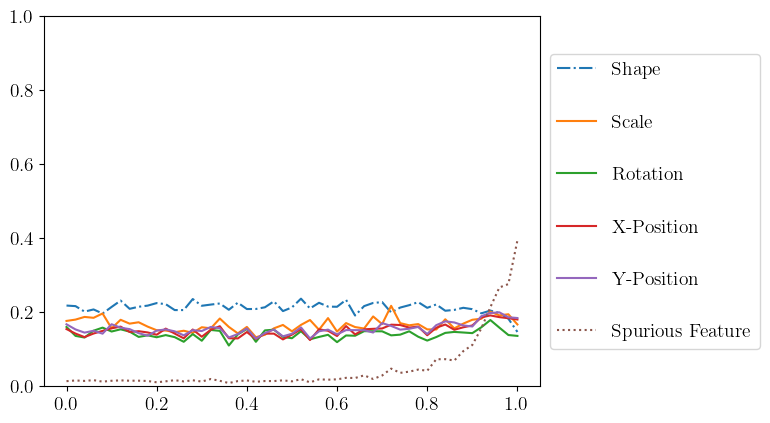
\includegraphics[height=4.5cm]{thesis_latex_template/pics/relevance_all_factors.png}
\end{minipage}\\

\begin{minipage}[t]{0.42\textwidth}
    \includegraphics[height=4.5cm]{thesis_latex_template/pics/mlc_all_factors_overlap.png}
\end{minipage}
\begin{minipage}[t]{0.49\textwidth}
    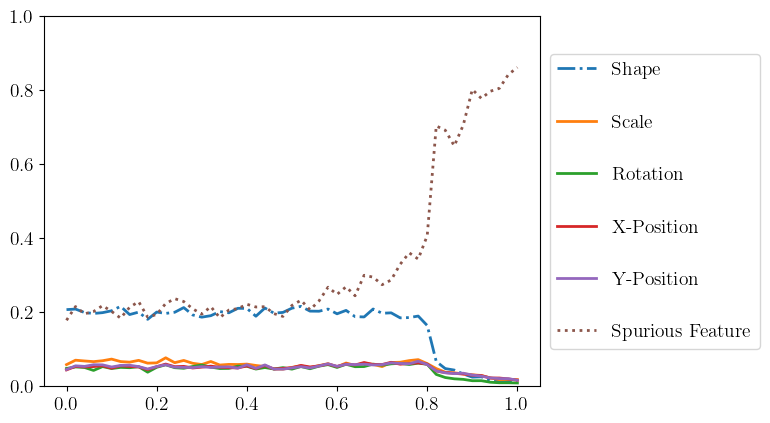
\includegraphics[height=4.5cm]{thesis_latex_template/pics/relevance_all_factors_overlap.png}
\end{minipage}
\caption{Reaction of models (and explanations) to other latent factors
left to right: logit change and relevance change, top: watermark scenario, bottom: pattern scenario }
\label{fig:other_latents_reaction}
\end{figure}

For the second \textit{pattern} dataset, the pixels within the shape are perturbed with Gaussian noise and for the case $W=1$ this pattern is blurred using a 3x3 Gaussian kernel with unit variance. All the other factors like the added noise term stay the same to the first scenario. We also note that we fix the random seed which initializes the noise term for each image and keep the order of images fed to the model during training fixed. 


\section{Model, Hyperparameters and Training}\label{appendix:model}
\subsection{Model Architecture}
For our analysis we decided on a model architecture that is small enough to train a few hundred times within a reasonable time frame but big enough to still have high performance for the scenarios and be comparable to the deep neural networks that local attribution methods are typically applied to.
We deemed 3 convolutional layers and one fully connected layer before the final output layer enough for our task. Notably, the layers have comparably few channels (8 or 6). The objective of creating such a narrow network was to be able to visually compare \textit{all} filters within a layer in order to identify the human-understandable concepts they (potentially redundantly) learned. 

\begin{lstlisting}[language=bash, label=lst:cnnmodel]

convolutional_layers: 
    0: Conv2d(in_channels=1, out_channels=8, kernel_size=3)
    1: MaxPool2d(kernel_size=2, stride=2)
    2: ReLU()
    3: Conv2d(in_channels=8, out_channels=8, kernel_size=5)
    4: MaxPool2d(kernel_size=2, stride=2)
    5: ReLU()
    6: Conv2d(in_channels=8, out_channels=8, kernel_size=7)
    7: ReLU()

linear_layers:
    0: Linear(in_features=392, out_features=6, bias=True)
    1: ReLU()
    2: Linear(in_features=6, out_features=2, bias=True)  

\end{lstlisting}

\subsection{Hyperparameter Choice}
The values for hyperparameters of the training process are optimized for accuracy with a rather short binary search. Finally, we train all models using the \verb|Adam| optimizer with a learning rate of \verb|0.001| using \verb|cross-entropy| loss as the objective to minimize. 
It is interesting to note that the learning rate has significantly different optimal values for highly biased models than completely unbiased ones and we therefore chose a compromise. We assume this to be due to the cost function becoming significantly different, arguably less complex, the more (\textit{information-theoretically}) useful the trivial watermark feature becomes to learn.
But importantly, those hyperparameters including the learning rate can not be changed over the course of training our set of models because it has been shown that explanation can depend on hyperparameters quite strongly \citep{Karimi2023}.
In our experiment we keep hyperparameters fixed and only intervene on the spurious-to-core feature ratio $\rho$. The only hyperparameter we choose to control for, is the random initialization of weights and biases. Usually, this is not identified as a hyperparameter. However, when using a seed to ensure that multiple models are initialized identically, while receiving differently generated data, it becomes possible to control for its effect like a causal variable. It can then be interpreted as the $\mathcal{U}$, or noise term, of the model.
As mentioned in the method section (\ref{section:model_zoo}), this seemed necessary because we observed the random initializations to have high variance in how they react to the spurious feature. This observation, and the apparent dependency of $\rho$ and the learning rate might also stand in relation to the findings of \cite{Karimi2023}, that the better a model performs, the more strongly the explanations seem to be affected by hyperparameters.

\subsection{Training and Accuracy}
We generate datasets by sampling the spurious-to-core feature ratio $\rho$ in 0.05 steps and training on the same dataset for instances of the model initialized with 16 different seeds. The training dataset contains 30 percent of all samples. Experimentally, much fewer samples seemed to be enough to achieve high accuracies. However, over-fitting is not a concern in our experiment and would, if anything, increase importance of the most important features. Taking even more samples would be too computationally expensive and harder to compare to real world problems where data is usually very limited. 
Due to the low complexity of this benchmark dataset, very high accuracies of over 95 percent are to be expected and also occur after comparably short training times for most models. \\


\subsection{Computational Setup}\label{appendix:setup}
The 1632 (816 for each scenario) models were trained on 4x NVIDIA A100 GPUs kindly provided by the Deutsches Klimarechenzentrum (DKRZ), which took about 40 hours in total, so on average 3 minutes per model. 
For the generation of 128x2x816 explanations about 30 minutes on a personal Dell XPS 13 laptop without dedicated graphics card was sufficient. All metrics were subsequently computed within minutes too. 

\section{Additional Results: Distance Metrics for Explanation Importance}\label{appendix:distance_metrics}

For relevance vectors the \textit{absolute} value is more sensitive to (arguably noise-like) small differences when $\rho$ is still small. This sensitivity seems to also be add to the distance value when $\rho$ is larger, although none of the metrics is able to recover the maximal importance of the watermark when $\rho = 1$ fully. 
Using the squared and cosine distance draws more attention to larger values, pulling the curve closer to the ground truth for small values of $\rho$. 
Both are only significantly departing from the true model importance for $\rho = 1.0$ and two spikes at $\rho = \{0.72, 0.82\}$. 

Similar results are found for the intervention on 8 attribution maps attributing importance to 64x64 pixels. 
Through smaller, probably noise-like variations the absolute and cosine distance measure slightly over-emphasize the importance of the watermark for low values of $\rho$. Note, that the squared distance for this higher-dimensional image set is very low as most pixels' attribution is zero. Therefore the squared metric is scaled to be within the interval of [0,1], i.e. divided by the maximum of all combinations of seeds and coupling ratios. 

\begin{figure}
    \centering
    \includegraphics[width=\textwidth]{thesis_latex_template/pics/m2_rel_comparison.png}
    \caption[Relevance Vector, Comparison of Metrics]{Comparison of distance metrics for relevance vectors (of 8 concepts in last convolutional layer).}
    \label{fig:m2_rel_comparison}
\end{figure}

\begin{figure}
    \centering
    \includegraphics[width=\textwidth]{thesis_latex_template/pics/m2_mac_comparison.png}
    \caption[Attribution Maps, Comparison of Metrics]{Comparison of distance metrics for 8 attribution maps (of last convolutional layer) each with dimension 64x64.}
    \label{fig:m2_mac_comparison}
\end{figure}


\section{Additional Benchmark Results: Pattern Scenario}\label{appendix:pattern_scenario}
Here we report additional results for the second dataset analogously to the first.
The second problem is constructed almost equivalently to the watermark problem but addresses the issue of spuriously correlated features that are not spatially separated from the target feature.
Instead of a watermark, the pattern within the shape is spuriously correlated with the shape itself. 
The relatively high accuracy on the training data (i.e. the biased data) of on average 95 percent and on anti-biased subsets can be seen in the figure in the result section \cref{fig:accuracy}.
The comparison of the 16 seeds analogous to \cref{fig:gt_over_seeds} is visualized in 
\cref{fig:compare_seeds_overlap}. In contrast to the first scenario, in the pattern scenario no seed seems to have been initialized at a position in the cost function which completely evades learning the bias feature.
This is a hint that the pattern feature is biasing the models stronger than the watermark feature.

\begin{figure}[!htb]
	\centering
	\label{fig:compare_seeds_overlap}
	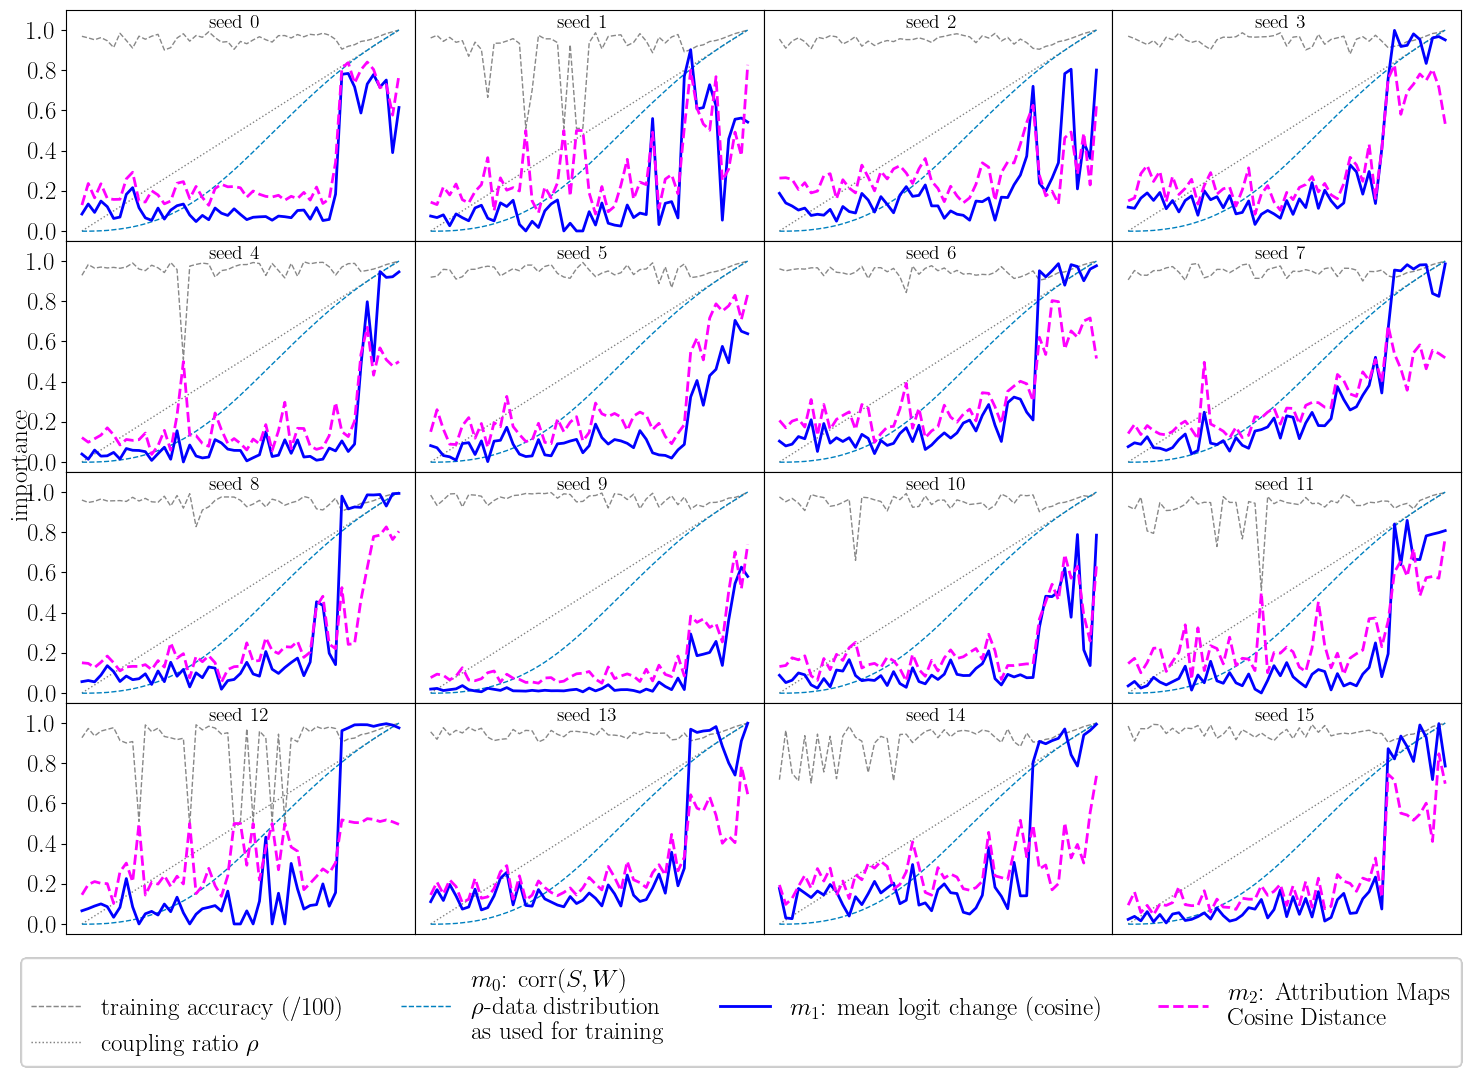
\includegraphics[width=\textwidth]{thesis_latex_template/pics/compare_seeds_overlap.png}
	\caption[Pattern Scenario Compare Seeds]{Comparing ground truth importance over 16 random initializations}
\end{figure}



\section{Correlation Independent of Coupling Ratio}

In our experiments we look at the correlation between the ground truth importance and the explained importance mostly by fixing values of $\rho$. Another visualization, relating $m_1$ and $m_2$ in scatter plots where each point represents one model, enables a different 
perspective. 

\begin{figure}[!htb]
	\centering
	\label{fig:scatter_plot_watermark}
	\includegraphics[height=\textheight]{thesis_latex_template/pics/scatter_plot_all_narrow.png}
	\caption[Correlation $m_1, m_2$ Watermark Scenario]{Scatter plots for the ground truth measure mean logit change $m_1$ and all different explanation importance measures $m_2$ for watermark scenario}
\end{figure}

\begin{figure}[!htb]
	\centering
	\label{fig:scatter_plot_pattern}
	\includegraphics[height=\textheight]{thesis_latex_template/pics/scatter_plot_all_narrow_overlap.png}
	\caption[Correlation $m_1, m_2$ Pattern Scenario]{Scatter plots for the ground truth measure mean logit change $m_1$ and all different explanation importance measures $m_2$ for pattern scenario}
\end{figure}